\documentclass[10pt,twocolumn]{article}

% ---------------------------------------------------------------------------
% Leave-Me-Alone: a binary-IP PTO optimizer. Short workshop-style paper.
% Build:  pdflatex main && bibtex main && pdflatex main && pdflatex main
% All numbers in Section 5 are \input from paper/tables/*.tex, generated by
% paper/experiments/make_tables.py from paper/results/results.json.
% ---------------------------------------------------------------------------

\usepackage[utf8]{inputenc}
\usepackage[T1]{fontenc}
\usepackage{amsmath,amssymb}
\usepackage{booktabs}
\usepackage{graphicx}
\usepackage{caption}
\usepackage{subcaption}
\usepackage{microtype}
\usepackage[hidelinks]{hyperref}
\usepackage[margin=0.85in]{geometry}
\usepackage{xcolor}
\usepackage{enumitem}

\graphicspath{{figures/}}

\title{\textbf{Leave Me Alone:}\\
A Binary Integer Program for Maximizing Continuous Time Off\\
from a Fixed Paid-Leave Budget}

\author{Wei Meng Ng\\
\small\texttt{github.com/ngweimeng/leave-me-alone}}

\date{}

\begin{document}
\maketitle

\begin{abstract}
Knowledge workers receive a fixed annual allotment of paid time off (PTO), yet
the \emph{value} of those days---measured as total continuous time away from
work---depends heavily on \emph{when} they are taken. Placing leave adjacent to
weekends and public holidays compounds short allotments into long, restorative
breaks. We formalize this as a binary integer program (IP) that maximizes the
number of \emph{break days} plus an adjacency bonus that rewards consecutive
breaks, subject to a leave budget and a fixed calendar of weekends and public
holidays. The model is compact---a single calendar year is roughly
$1.1\times10^{3}$ binary variables and $1.5\times10^{3}$ constraints---and
solves to proven optimality in milliseconds. We implement the model behind a
common solver interface and benchmark four production engines spanning two
algorithmic paradigms: LP-based branch-and-cut (FICO Xpress, Gurobi, SCIP) and
constraint programming over a SAT core (Google OR-Tools CP-SAT). All four
recover the same optimal objective, but they routinely return
\emph{different, equally optimal} schedules, demonstrating a highly degenerate
solution space. We then expose a subtle modeling pitfall: the adjacency weight
$\alpha$, which looks like a tunable ``vacation style'' knob, is really a
\emph{threshold}---any positive value clusters maximally and further increases
do nothing. Controlling break \emph{length} instead requires a hard
constraint, a max-stretch cap, which we add and show to be the faithful dial
$\alpha$ only appears to be. Finally we show achievable break structure varies
markedly across national holiday calendars. The system is open source and ships
as an interactive planner.
\end{abstract}

% ===========================================================================
\section{Introduction}
% ===========================================================================

Annual leave is a scarce, use-it-or-lose-it resource. A typical employee plans
PTO informally---a Friday here, a bridge day there---and rarely with respect to
the full year's calendar of weekends and public holidays. Yet the difference
between a naive and an optimized placement is large: the same fifteen days,
placed well, can produce several week-plus continuous breaks rather than a
scatter of isolated long weekends.

This is a combinatorial optimization problem with a clean structure. The
calendar is fixed; weekends and public holidays are ``free'' break days; the
only decisions are which weekdays to spend leave on, subject to a budget. The
objective---total continuous time off---rewards \emph{clustering} leave against
the free days. We make this precise as a binary integer program and study both
its mathematical behavior and its computational profile across solvers.

\paragraph{Contributions.}
\begin{enumerate}[leftmargin=1.4em,itemsep=2pt,topsep=2pt]
  \item A compact binary-IP formulation of PTO placement with a linearized
        adjacency reward and an optional max-stretch cap on break length
        (Section~\ref{sec:model}).
  \item A solver-agnostic implementation and a reproducible benchmark of four
        engines across two paradigms (Section~\ref{sec:impl}--\ref{sec:results}).
  \item Empirical findings: (i) all engines tie on objective but disagree on
        \emph{which} optimal schedule they return---the optimum is highly
        non-unique; (ii) the adjacency weight $\alpha$ is a \emph{threshold},
        not a dial---a soft reward that looks tunable but behaves like a switch;
        (iii) a hard max-stretch constraint is the genuine length control, and
        it reshapes the schedule while leaving total time off invariant;
        (iv) free-license size caps, not algorithmic limits, bind at multi-year
        horizons; and (v) holiday calendars differ enough that the same budget
        buys very different break structure across countries.
\end{enumerate}

% ===========================================================================
\section{Related Work}
% ===========================================================================

Integer programming and branch-and-bound are foundational tools of operations
research~\cite{land1960automatic,wolsey1999integer}, and the art of encoding
logical conditions as linear constraints is well
documented~\cite{williams2013model}. The practical tractability of
mixed-integer programming has improved by orders of magnitude over recent
decades through advances in both algorithms and
solvers~\cite{bixby2012brief,achterberg2013mixed}. Our model exercises a
classic modeling pattern---linearizing a logical AND ($a = x \wedge y$) over
binaries---and is small enough that the interesting questions are not about
tractability but about \emph{solution structure} and \emph{cross-solver
behavior}.

Personnel and shift scheduling are mature IP application areas, but they
typically optimize an employer's coverage subject to labor rules. The problem
here is the dual, employee-facing one: a single individual maximizing the
restorative value of a fixed leave budget against a public calendar. We are not
aware of a formal treatment of this specific objective, though ``bridge day''
heuristics are folklore. We rely on the open-source \texttt{holidays}
library~\cite{pythonholidays} for national calendars and deliver the tool as a
\texttt{Streamlit} application~\cite{streamlit}.

% ===========================================================================
\section{Problem Formulation}
\label{sec:model}
% ===========================================================================

\subsection{Sets and parameters}
Let $D = (d_1, \dots, d_n)$ be the ordered set of dates in the planning
horizon, and write $d^{+}$ for the successor of $d$ in $D$. Let
$H \subseteq D$ be the dates that are \emph{fixed breaks}: weekends (Saturday or
Sunday) or public holidays. Let $P \subseteq D$ be dates pre-booked as leave.
The parameters are the leave budget $L \in \mathbb{Z}_{\ge 0}$, the adjacency
weight $\alpha \in \mathbb{R}_{\ge 0}$, and an optional cap
$K \in \mathbb{Z}_{\ge 1} \cup \{\infty\}$ on the length of any continuous break
($K=\infty$ means uncapped).

\subsection{Decision variables}
For each $d \in D$ we introduce three binary variables:
\begin{align}
  l_d &\in \{0,1\}, && \text{leave is taken on day } d,\\
  b_d &\in \{0,1\}, && \text{day } d \text{ is a break day},\\
  a_d &\in \{0,1\}, && \text{both } d \text{ and } d^{+} \text{ are breaks},
\end{align}
where $a_d$ is defined for every $d$ that has a successor.

\subsection{Objective}
We maximize the number of break days plus a weighted count of adjacent break
pairs:
\begin{equation}
  \max \;\; \sum_{d \in D} b_d \;+\; \alpha \sum_{d \in D \setminus \{d_n\}} a_d .
  \label{eq:obj}
\end{equation}
The first term counts total time off; the second rewards \emph{contiguity}, so
that for a fixed number of break days the model prefers fewer, longer stretches.

\subsection{Constraints}
\begin{align}
  l_d &= 1, & &\forall d \in P, \label{eq:prebook}\\
  \sum_{d \in D} l_d &\le L, & & \label{eq:budget}\\
  b_d &= 1, & &\forall d \in H, \label{eq:fixed}\\
  b_d &\le l_d, & &\forall d \in D \setminus H, \label{eq:weekday}\\
  a_d &\le b_d, \quad a_d \le b_{d^{+}}, & & \label{eq:and1}\\
  a_d &\ge b_d + b_{d^{+}} - 1, & & \label{eq:and2}\\
  \sum_{d \in W} b_d &\le K, & &\forall W \in \mathcal{W}_K. \label{eq:cap}
\end{align}
Constraint~\eqref{eq:prebook} honors commitments; \eqref{eq:budget} enforces the
budget; \eqref{eq:fixed} makes weekends and holidays free breaks;
\eqref{eq:weekday} lets a weekday become a break \emph{only} if leave is spent
on it. The triple \eqref{eq:and1}--\eqref{eq:and2} is the standard
linearization of the logical AND $a_d = b_d \wedge b_{d^{+}}$: the first two
inequalities force $a_d = 0$ unless both neighbors are breaks, and the third
forces $a_d = 1$ when they are.

\paragraph{Max-stretch cap.}
Constraint~\eqref{eq:cap} bounds break \emph{length}. When $K<\infty$, no run of
$K{+}1$ consecutive break days is allowed: for each length-$(K{+}1)$ window of
consecutive dates we require at most $K$ of them to be breaks. The window set
$\mathcal{W}_K$ deliberately \emph{excludes} windows whose days are all fixed
breaks (all weekend/holiday): such a window is forced to $K{+}1$ by
\eqref{eq:fixed} and capping it would make the model infeasible. Excluding it
leaves a pre-existing forced holiday run (e.g.\ Japan's Golden Week) untouched
while still preventing \emph{leave} from creating or extending a run beyond $K$.
This keeps the model feasible for every $K\ge 1$.

\subsection{Structural remarks}
\label{sec:structure}
Two properties drive the empirical results.

\paragraph{Break count is budget-determined.}
Because every weekday break requires one unit of leave \eqref{eq:weekday} and
fixed breaks are constant \eqref{eq:fixed}, \emph{any} feasible schedule that
spends the full budget achieves the same first-term value
$\sum_d b_d = |H| + L$ (assuming $L$ weekdays are available, which holds for
realistic budgets). The first term of the objective is therefore effectively a
constant at optimality. \emph{All optimization pressure flows through the
adjacency term}---the model's real job is to \emph{arrange} a fixed number of
break days, not to choose how many.

\paragraph{$\alpha$ is a threshold, not a dial.}
Given the above, maximizing $\sum_d a_d$ for a fixed break count is equivalent
to \emph{minimizing the number of disjoint break stretches} (each stretch of
length $k$ contributes $k-1$ adjacencies, so total adjacencies
$= (\text{break days}) - (\text{\# stretches})$). Once $\alpha > 0$ is large
enough to make a single merged stretch preferable to two separate ones, further
increases change nothing. We confirm this empirically in
Section~\ref{sec:results}: the schedule is identical for
$\alpha \in \{1.5, 2, 4, 8\}$. The practical consequence is that $\alpha$
\emph{cannot} express a preference for breaks of a particular length---it only
chooses between ``fragment'' ($\alpha=0$) and ``cluster maximally''
($\alpha>0$). To control break \emph{length}, one needs the cap $K$
\eqref{eq:cap}, which we show in Section~\ref{sec:results} acts as the genuine
dial that $\alpha$ is not.

% ===========================================================================
\section{Implementation}
\label{sec:impl}
% ===========================================================================

The model is implemented in Python behind a single abstract interface,
\texttt{LeaveSolver}, that takes an immutable \texttt{LeaveProblem} (dates,
holidays, budget, $\alpha$, pre-booked days, and the cap $K$) and returns a
solution plus measured statistics. The feasible window set $\mathcal{W}_K$ is
computed once on the problem and shared by all backends, so each engine adds the
cap as a single constraint loop. Four concrete backends translate the
\emph{same} model into their native APIs:
\begin{itemize}[leftmargin=1.4em,itemsep=2pt,topsep=2pt]
  \item \textbf{FICO Xpress}~\cite{ficoxpress} --- LP branch-and-cut; free
        Community Edition capped near $5000$ rows/columns.
  \item \textbf{Gurobi}~\cite{gurobi} --- LP branch-and-cut; the free
        \texttt{pip} license is capped at $2000$ variables and $2000$
        constraints.
  \item \textbf{SCIP}~\cite{bestuzheva2023scip} --- LP branch-and-cut; fully
        open source, no size cap.
  \item \textbf{OR-Tools CP-SAT}~\cite{perron2023cpsat} --- constraint
        programming over a SAT core with a parallel portfolio of strategies;
        open source, no cap. A \emph{different paradigm} from the LP engines,
        which makes it the most interesting point of comparison.
\end{itemize}
A registry detects which backends are importable and licensed and exposes only
those; a benchmark harness solves one problem with all of them and flags when
their schedules diverge. National holiday calendars come from the
\texttt{holidays} library~\cite{pythonholidays}.

% ===========================================================================
\section{Experiments}
\label{sec:results}
% ===========================================================================

All experiments run the production solver code. The harness
(\texttt{paper/experiments/run\_experiments.py}) emits a single JSON file from
which every table below is generated automatically, so the reported numbers
cannot drift from the measurements.

\paragraph{Setup.}
Hardware: Apple silicon (\texttt{arm64}), macOS. Solver versions: Xpress~9.8.1,
Gurobi~12.0.3, SCIP via \texttt{pyscipopt}~6.2.1, OR-Tools~9.15. Each engine
runs in its \emph{default} configuration (notably, CP-SAT keeps its multi-thread
portfolio). Timings report the best of seven runs to reduce noise. The
canonical instance is the United States, 2026, $L=15$, $\alpha=1.5$
(``balanced'' preset)---$365$ days, $12$ public holidays.

\subsection{Solver comparison on the canonical instance}
Table~\ref{tab:comparison} reports time and objective for each backend on the
identical model.

\begin{table}[t]
  \centering
  \caption{Canonical instance (US 2026, $L=15$, $\alpha=1.5$). All backends
  reach the same optimal objective; times are best-of-seven.}
  \label{tab:comparison}
  \small
  \begin{tabular}{lrrrrr}
    \toprule
    Solver & Vars & Cons & Obj & Best & Med.\\
           &      &      &     & (ms) & (ms)\\
    \midrule
    Xpress & 1094 & 1458 & 251.5 & 10.2 & 10.6 \\
Gurobi & 1094 & 1458 & 251.5 & 9.6 & 9.8 \\
SCIP & 1094 & 1458 & 251.5 & 132.5 & 134.2 \\
OR-Tools (CP-SAT) & 1094 & 1458 & 251.5 & 28.2 & 56.4
 \\
    \bottomrule
  \end{tabular}
\end{table}

\paragraph{Finding 1: identical objective, divergent schedules.}
Every backend attains the same optimum, yet the benchmark flags that the
\emph{chosen leave days differ between engines}. This is a direct consequence of
the degeneracy noted in Section~\ref{sec:structure}: with break count fixed and
many ways to arrange the same number of stretches, the optimal face of the
polytope is high-dimensional, and each engine's tie-breaking lands on a
different vertex. For the user, any of these schedules is equally good; for the
benchmark, divergence is the expected signal, not an anomaly.

\subsection{Scaling and the binding constraint}
We grow the horizon from three months to four years (scaling the budget at
$\approx 25$ days/year) and impose a per-solve wall-clock cap.
Table~\ref{tab:scaling} and Figure~\ref{fig:scaling} report the result.

\begin{table}[t]
  \centering
  \caption{Best solve time (ms) vs.\ horizon. ``---'' marks a free-license size
  cap (the model exceeds the licensed limit), \emph{not} a timeout. A
  $\sim$ prefix marks a horizon where the engine did not prove optimality in
  every run within the cap.}
  \label{tab:scaling}
  \small
  \setlength{\tabcolsep}{4pt}
  \begin{tabular}{lrrrrrr}
    \toprule
    Horizon & Days & Vars & Xpr. & Gur. & SCIP & OR-T.\\
    \midrule
    3 months & 90 & 269 & 2.2 & 1.0 & 10.4 & 7.5 \\
6 months & 182 & 545 & 5.5 & 4.3 & 38.9 & 13.1 \\
1 year & 365 & 1094 & 6.6 & 6.4 & 54.2 & 28.4 \\
2 years & 730 & 2189 & \textemdash & \textemdash & 125.4 & 226.3 \\
3 years & 1095 & 3284 & \textemdash & \textemdash & 331.3 & $\sim$3832.5 \\
4 years & 1460 & 4379 & \textemdash & \textemdash & 1458.9 & $\sim$1708.1
 \\
    \bottomrule
  \end{tabular}
\end{table}

\begin{figure}[t]
  \centering
  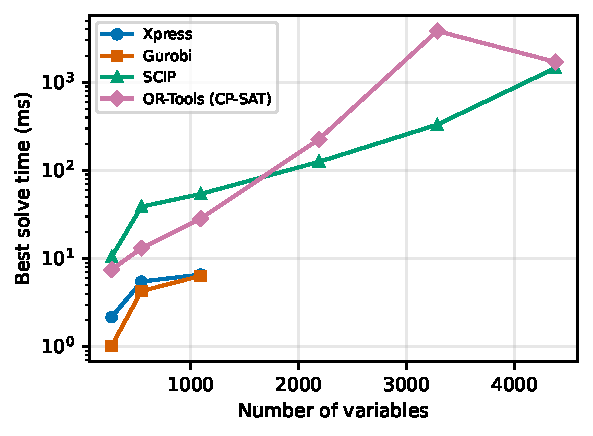
\includegraphics[width=\linewidth]{fig_scaling.pdf}
  \caption{Solve time vs.\ problem size (log scale). The commercial engines
  under free licenses stop at their size caps; the open-source engines scale
  through multi-year horizons.}
  \label{fig:scaling}
\end{figure}

\paragraph{Finding 2: licenses bind before algorithms do.}
On the realistic single-year instance all four engines finish in tens of
milliseconds. As the horizon grows, the \emph{first} thing to fail is not solver
speed but the free-license size caps: Gurobi's $2000$-variable limit is exceeded
at two years and Xpress's $\sim$5000-row limit at four. The uncapped open-source
engines (SCIP, CP-SAT) solve all horizons. CP-SAT's parallel portfolio shows
higher proof-time variance on the largest instances---it reliably \emph{finds}
the optimum quickly but occasionally takes longer to \emph{prove} it---whereas
SCIP's branch-and-cut proof time grows smoothly. For the intended use case
(a single year), all of this is moot; the practical lesson is that an
open-source backend removes the only real limit.

\subsection{The adjacency weight is a threshold control}
Table~\ref{tab:alpha} sweeps $\alpha$ on the canonical instance and reports the
resulting break structure.

\begin{table}[t]
  \centering
  \caption{Effect of the adjacency weight $\alpha$ (US 2026, $L=15$). Break and
  leave counts are invariant; only the \emph{arrangement} responds, and it
  saturates immediately.}
  \label{tab:alpha}
  \small
  \setlength{\tabcolsep}{4pt}
  \begin{tabular}{rrrrrl}
    \toprule
    $\alpha$ & Brk & Lv & Str. & Long. & Stretch sizes\\
    \midrule
    0.0 & 130 & 15 & 54 & 15 & 15, 5, 4, 3, 3, 3, 3, 3 \\
1.5 & 130 & 15 & 49 & 9 & 9, 9, 9, 4, 4, 3, 3, 3 \\
2.0 & 130 & 15 & 49 & 9 & 9, 9, 9, 4, 4, 3, 3, 3 \\
4.0 & 130 & 15 & 49 & 9 & 9, 9, 9, 4, 4, 3, 3, 3 \\
8.0 & 130 & 15 & 49 & 9 & 9, 9, 9, 4, 4, 3, 3, 3
 \\
    \bottomrule
  \end{tabular}
\end{table}

\begin{figure}[t]
  \centering
  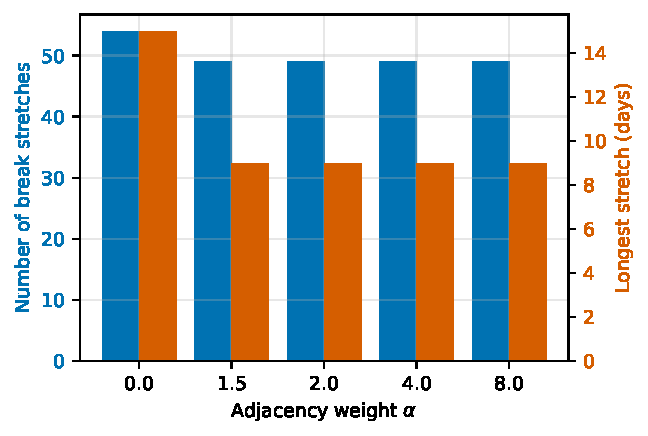
\includegraphics[width=\linewidth]{fig_alpha.pdf}
  \caption{Number of break stretches (left axis) and longest stretch (right
  axis) vs.\ $\alpha$. At $\alpha=0$ the arrangement is unconstrained; any
  $\alpha$ above the threshold yields the same clustered schedule.}
  \label{fig:alpha}
\end{figure}

\paragraph{Finding 3: shape, not size, and it saturates.}
As predicted in Section~\ref{sec:structure}, the number of break days and leave
days is constant across $\alpha$. At $\alpha=0$ the model is indifferent to
contiguity and returns a fragmented schedule; any positive $\alpha$ past the
threshold collapses the schedule to the same maximally clustered arrangement
(fewest stretches, longest runs). A continuous appearance of control hides a
discrete reality: $\alpha$ chooses only between ``fragment'' and ``cluster,''
never between break \emph{lengths}. This is a cautionary modeling result---a
soft reward in the objective looks like a tunable knob but behaves like a
switch.

\subsection{The max-stretch cap is the real dial}
The fix follows directly from Finding~3: to control break length one must
constrain it, not reward it. Table~\ref{tab:maxstretch} and
Figure~\ref{fig:maxstretch} sweep the cap $K$ \eqref{eq:cap} on the canonical
instance.

\begin{table}[t]
  \centering
  \caption{Effect of the max-stretch cap $K$ (US 2026, $L=15$, $\alpha=1.5$).
  Break and leave counts stay constant, but unlike $\alpha$ the cap reshapes the
  schedule continuously: it directly sets the longest run.}
  \label{tab:maxstretch}
  \small
  \setlength{\tabcolsep}{4pt}
  \begin{tabular}{rrrrrl}
    \toprule
    $K$ & Brk & Lv & Str. & Long. & Stretch sizes\\
    \midrule
    4 & 130 & 15 & 53 & 4 & 4, 4, 4, 4, 4, 4, 4, 3 \\
6 & 130 & 15 & 52 & 6 & 6, 5, 5, 4, 4, 3, 3, 3 \\
9 & 130 & 15 & 49 & 9 & 9, 9, 9, 4, 4, 3, 3, 3 \\
none & 130 & 15 & 49 & 9 & 9, 9, 9, 4, 4, 3, 3, 3
 \\
    \bottomrule
  \end{tabular}
\end{table}

\begin{figure}[t]
  \centering
  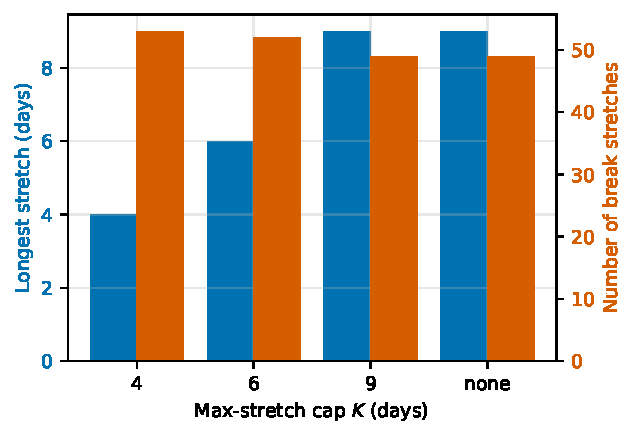
\includegraphics[width=\linewidth]{fig_max_stretch.pdf}
  \caption{Longest stretch (left) and number of stretches (right) vs.\ the cap
  $K$. Tightening $K$ trades a few long blocks for more short ones; the longest
  run tracks $K$ exactly until the uncapped optimum is reached.}
  \label{fig:maxstretch}
\end{figure}

\paragraph{Finding 4: constrain length, don't reward it.}
With $\alpha$ held at a single positive value, varying $K$ produces genuinely
distinct schedules---$K{=}4$ yields a fabric of long-weekends, $K{=}9$ a few
week-long blocks, and the uncapped case the longest runs the calendar allows---
all while spending the identical budget and achieving the identical break-day
count. The cap is the legible, faithful control the UI presets need; the
adjacency weight, fixed to ``on,'' merely ensures the days within each capped
window stay contiguous. Total time off is invariant to $K$; only its
\emph{distribution} changes, which is exactly the user-facing choice.

\subsection{Holiday leverage across countries}
Finally we hold the budget fixed ($L=15$, 2026) and vary the country, so only
the public-holiday calendar changes. Table~\ref{tab:leverage} and
Figure~\ref{fig:leverage} report the achievable structure.

\begin{table}[t]
  \centering
  \caption{Same budget ($L=15$, 2026), different national calendars. Weekday
  holidays (those not already on a weekend) are what PTO can leverage; the
  longest achievable continuous break varies widely.}
  \label{tab:leverage}
  \small
  \setlength{\tabcolsep}{4pt}
  \begin{tabular}{lrrrrr}
    \toprule
    Ctry & Hol & Base & Break & Extra & Long.\\
    \midrule
    JP & 18 & 121 & 136 & 15 & 16 \\
DE & 9 & 111 & 126 & 15 & 11 \\
GB & 7 & 110 & 125 & 15 & 10 \\
SG & 14 & 114 & 129 & 15 & 10 \\
FR & 11 & 113 & 128 & 15 & 10 \\
US & 12 & 115 & 130 & 15 & 9 \\
IN & 16 & 116 & 131 & 15 & 9 \\
BR & 10 & 113 & 128 & 15 & 9
 \\
    \bottomrule
  \end{tabular}
\end{table}

\begin{figure}[t]
  \centering
  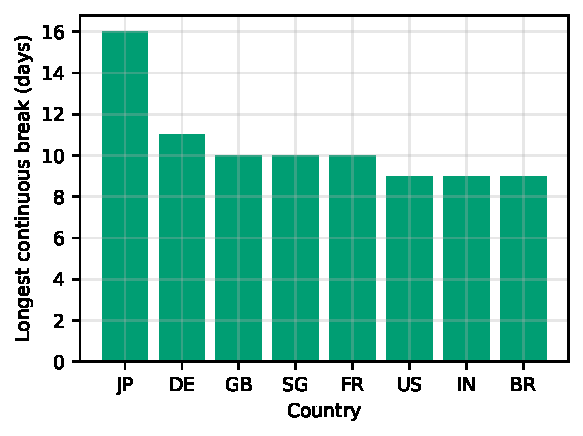
\includegraphics[width=\linewidth]{fig_leverage.pdf}
  \caption{Longest achievable continuous break by country for a fixed
  $15$-day budget. The number and weekday-alignment of public holidays, not the
  budget, drives the ceiling.}
  \label{fig:leverage}
\end{figure}

\paragraph{Finding 5: the calendar sets the ceiling.}
Each PTO day extends a break by one day, so total break days move in lockstep
with the budget regardless of country. What differs is the \emph{best continuous
stretch} the calendar permits: where several public holidays cluster near a
weekend, a modest budget bridges them into a long block; where holidays are
sparse or fall on weekends, the same budget yields shorter runs. The binding
resource for \emph{quality} of time off is the national calendar, not the
allotment.

% ===========================================================================
\section{Discussion and Limitations}
% ===========================================================================

The model deliberately optimizes a single, legible objective. Beyond the
max-stretch cap, it does not model preferences over \emph{when} in the year
breaks fall, a \emph{minimum} stretch length, school terms, or team blackout
periods; the formulation has ample headroom (a year is well under any solver's
free cap) to add such constraints, and the window pattern of \eqref{eq:cap}
extends naturally (e.g.\ a minimum-stretch or season-preference variant). The
degeneracy we observe is a feature for the user---many equally good answers---but
means that ``the'' optimal schedule is not well defined; a secondary objective
(e.g.\ preferring breaks in summer) would select among ties deterministically.
Finally, our holiday data inherits any inaccuracies of the upstream library.

% ===========================================================================
\section{Conclusion}
% ===========================================================================

We cast the placement of a fixed PTO budget as a compact binary integer program
that maximizes continuous time off by clustering leave against weekends and
public holidays. The model solves instantly at realistic scale on any of four
production solvers, which agree on value but not on schedule---a textbook
degenerate optimum. We showed that break count is budget-determined; that the
adjacency weight is a \emph{threshold} masquerading as a tunable knob, so break
\emph{length} must be governed by a hard max-stretch cap rather than a soft
reward; that free licenses rather than algorithms bind at long horizons; and
that national holiday calendars set the ceiling on achievable break quality. The
soft-reward-versus-hard-constraint lesson generalizes beyond this problem: when
a quantity is determined by a budget, rewarding a correlate of the desired shape
in the objective can silently collapse to a switch, and the property one
actually wants is better stated as a constraint. The system is open source and
usable today as an interactive planner.

\bibliographystyle{plain}
\bibliography{references}

\end{document}
